\documentclass[10pt,foldmark,tumble]{leaflet}
\usepackage[utf8]{inputenc}
\usepackage{mathptmx}
\usepackage{url}
\usepackage{graphicx,txfonts}
\usepackage[dvipsnames,usenames]{color}
\usepackage{dirtytalk}
\usepackage{anyfontsize}

\usepackage[framemethod=TikZ]{mdframed}
\mdfdefinestyle{MyFrame}{%
    linecolor=blue,
    outerlinewidth=2pt,
    roundcorner=20pt,
    innertopmargin=\baselineskip,
    innerbottommargin=\baselineskip,
    innerrightmargin=20pt,
    innerleftmargin=20pt,
    backgroundcolor=gray!30!white}

\mdfdefinestyle{titframe}{%
    linecolor=red,
    outerlinewidth=1pt,
    roundcorner=5pt,
    innertopmargin=\baselineskip / 4,
    innerbottommargin=\baselineskip / 2,
    innerrightmargin=10pt,
    innerleftmargin=30pt,
    backgroundcolor=orange!30!white}

\newcommand{\tit}[1]{\section{
\includegraphics{item.png}#1}}
\newcommand{\love}{{\color{red}\ensuremath\varheartsuit}}
\newcommand{\fsfeg}{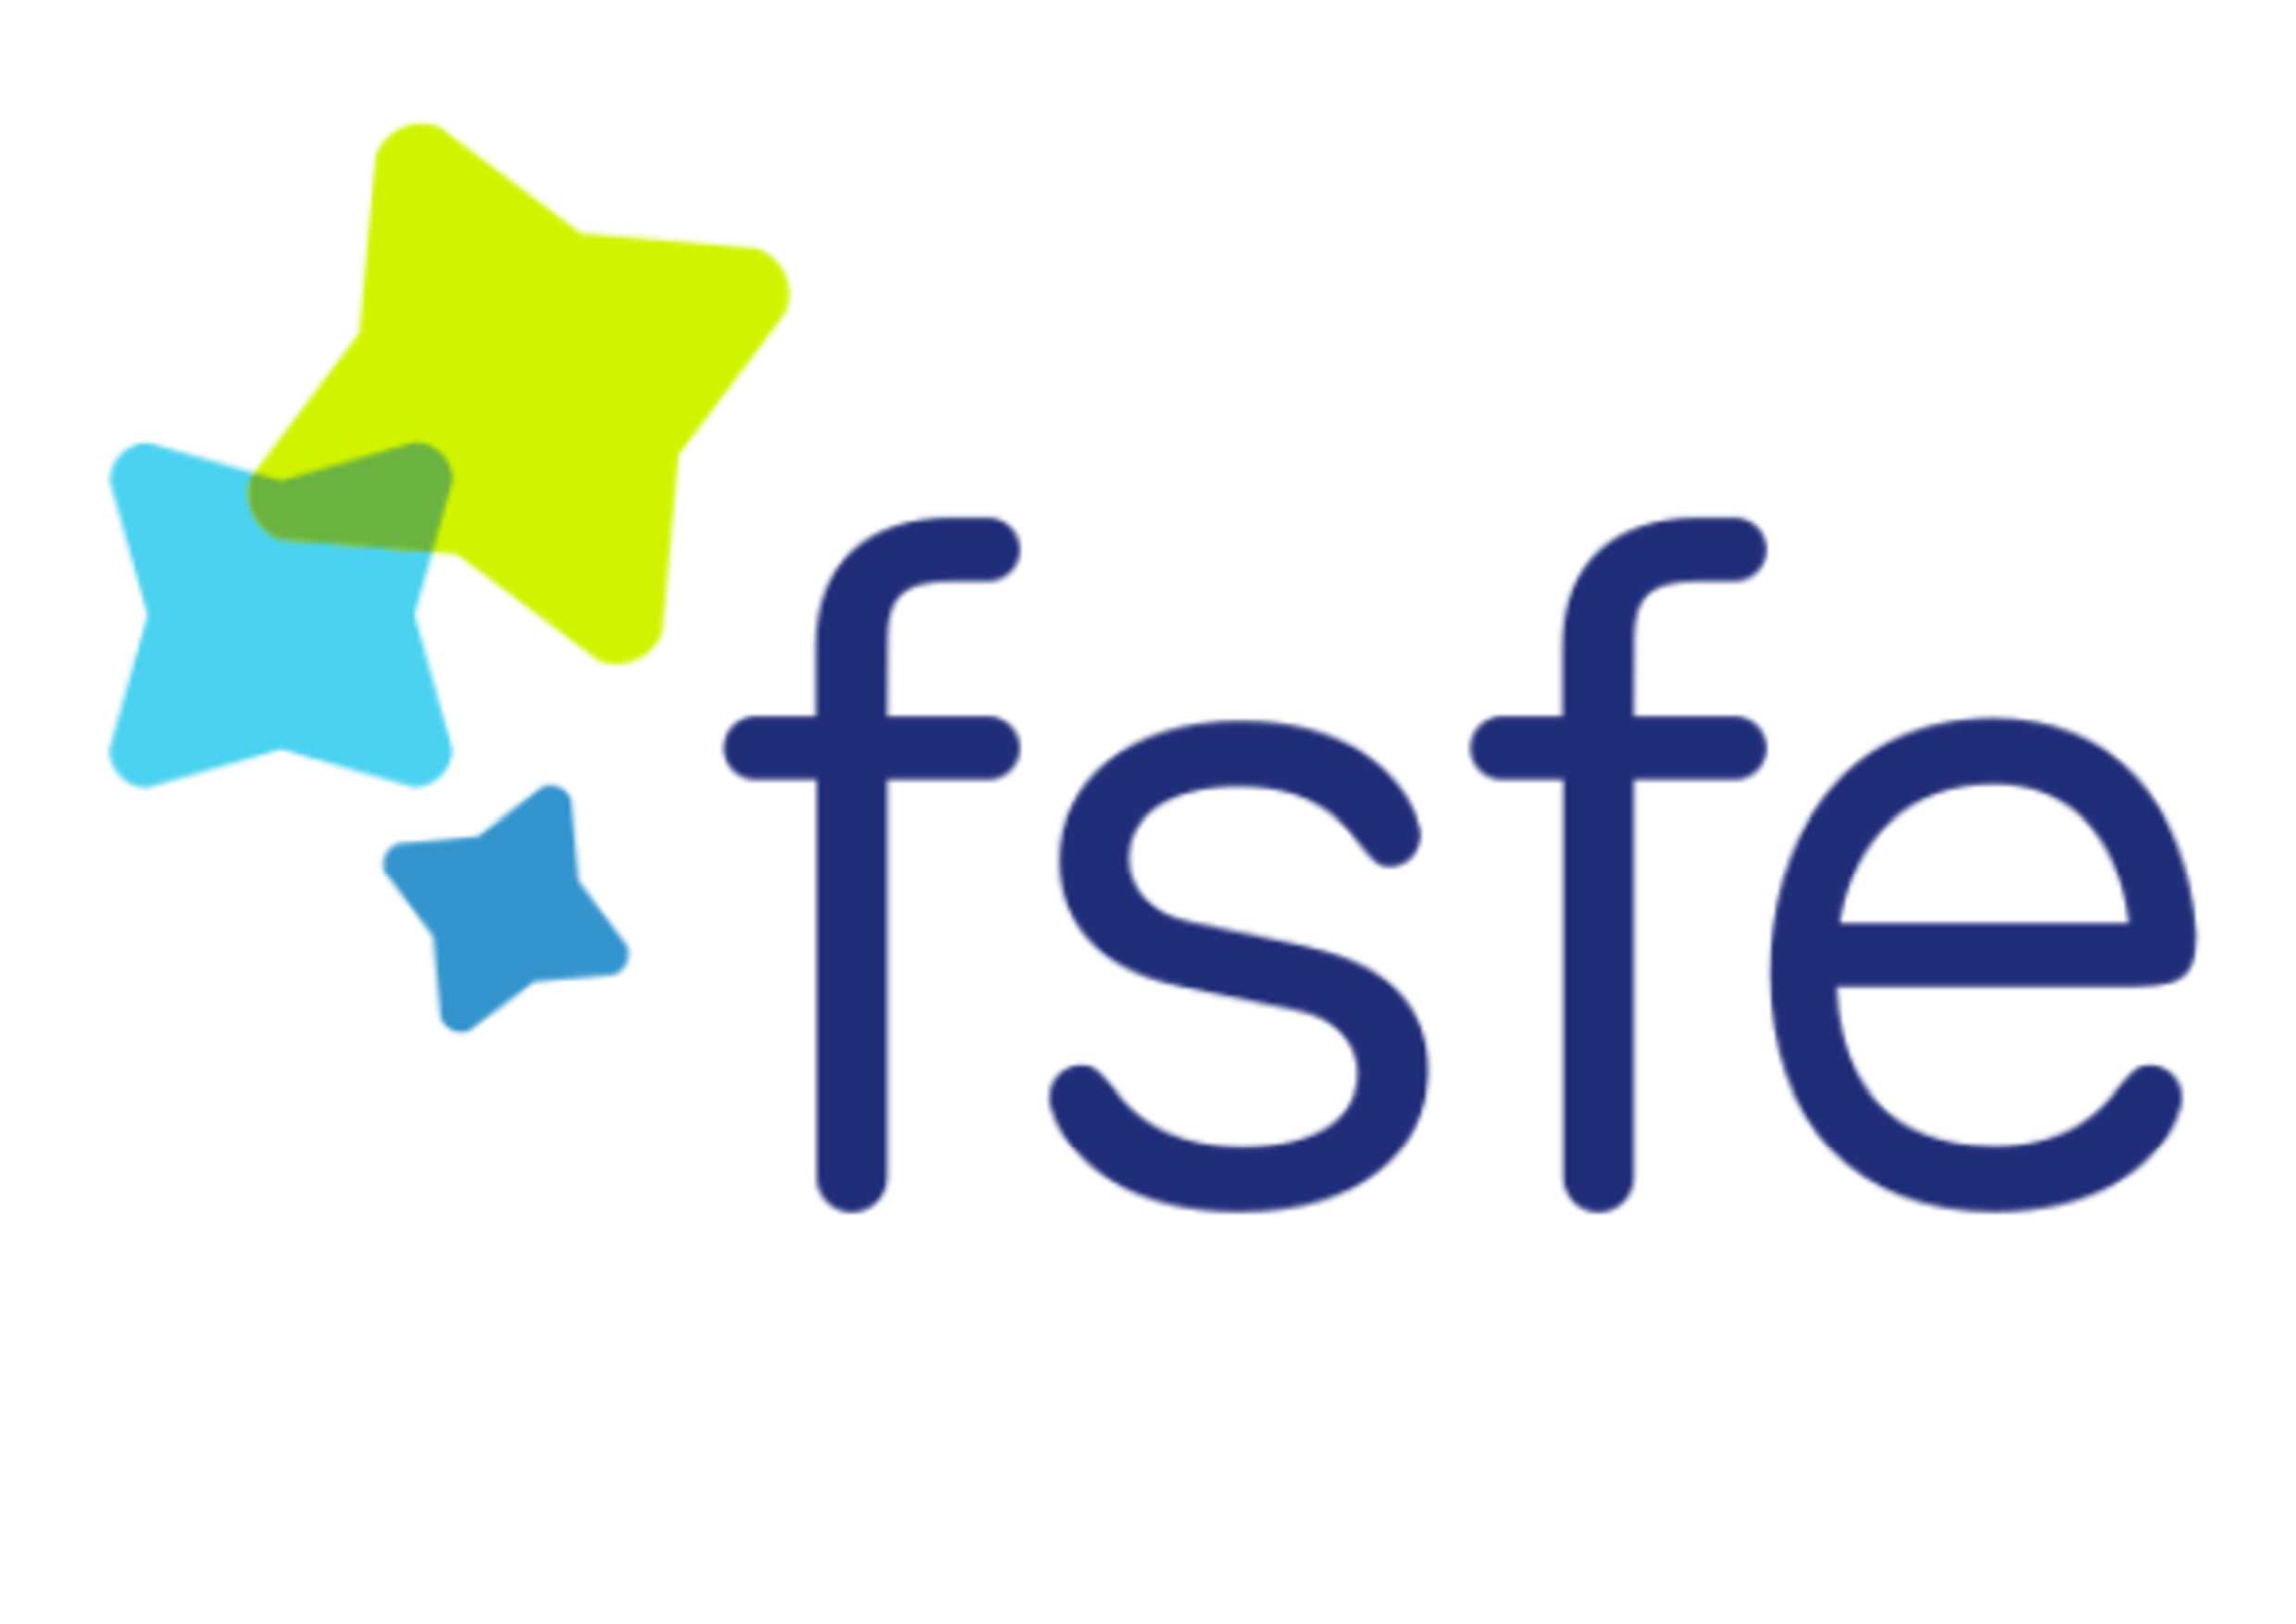
\includegraphics[scale=0.10]{fsfe.pdf}{\fontsize{70}{60} \love}{\Huge Galego}}

\CutLine*{1}% Dotted line without scissors
\CutLine*{6}
%%\CutLine{6}%  Dotted line with scissors

%%\AddToBackground{6}{%  Background of a small page
%%  \put(0,0){\textcolor{Cyan}{\rule{\paperwidth}{\paperheight}}}}


\begin{document}

\begin{flushright}
{\Huge Eu{\color{red}\love}Galego!} 
\end{flushright}

\fsfeg

\section{
\includegraphics{item.png}Acerca da FSFE}

As persoas da Fundación do Software Libre de Europa (FSFE) consideránse europeus de diferentes culturas co obxectivo común de cooperar entre culturas e desenvolver unhaa cultura común de cooperación dende un nivel local até un global.

A FSFE é unha organización non gubernamental sen ánimo de lucro e tamén unha rede integrada nunha rede global de persoas con obxectivos e visións comúns. As persoas da FSFE só se representan a si propios e ao seu traballo. Ese traballo a prol da liberdade en todos os aspectos da sociedade dixital é o que os define.

Os principios da FSFE son os de democracia, transparencia, pluralismo, consistencia, confiabilidade e concentración.

O traballo dos voluntarios é o fundamental sobre o que descansa todo. Existen diferentes niveis de implicación e todo o mundo é benvido a participar permanente, regular ou ocasionalmente nas actividades da FSFE.

Os membros da asociación son propostos normalmente por membros das equipas e das organizacións asociadas dos países e aprobadas pola asamblea xeral da asociación FSFE.

A asociación FSFE é fundamentalmente democrática. Todas as partes da FSFE (membros da asociación, das equipas...) son benvenidas a participar no proceso de toma de decisións.

Ainda que as contribucións valuntarias son os alicerces do traballo da FSFE hai tarefas que precisan dedicación a tempo completo desenvolvido por empregados que realizan únicamente traballos de producción e non forman parte dos procesos xerais de toma de decisións.

  \subsection{Procesos de decisión}

As persoas da Fundación do Software Libre de Europa cren no consenso, no que basean o seu traballo así como no compromiso dos membros activos. 

Mais en ocasións compre accións rápidas e decisivas por iso estableceuse a asociación FSFE e os seus comités executivos ampliados en niveis europeu e nacional que aportan estruturas e procedimientos xestionados e controlados mediante procesos democráticos.

Este plantexamento adoptouse na procura dunha estrutura que permitise a transparencia, o pluralismo e a participación, sendo ao mesmo tempo tan sinxela como for posible.

Asegura a posibilidade de participación de todas as partes da FSFE, os membros da asociación, das equipas e das organizacións asociadas poden todos participar. Deste xeito a Fundación do Software Libre de Europa pode actuar rápidamente cando ser necesario e manter unha forte consistencia de organización a longo prazo.

\tit{As traduccións na FSFE}

A Free Software Foundation Europe é unha organización internacional con obxectivo de chegar a tanta xente como sexa posible e incluir a toda esa xenta nas actividades da FSFE para promover, axuda e dar soporte ao movemento do Software Libre. Para conseguilo a FSFE quere facer accesible en diferentes idiomas toda a información publicada tanto en textos como na propia web.

Moitas das traduccións da FSFE empreganse en outros proxectos de Software Libre así que axudar na traducción na FSFE reforza a comunidade do Software Libre a largo prazo e dalle á xente, sen importar o seu idioma ou nacionalidade, unha oportunidade de aprender máis sobre o Software Libre.

Traducir e revisar textos é unha contribución moi importante ao traballo da FSFE e unha oportunidade excelente de formar parte das actividades da FSFE sen ter obligacións a largo prazo.

\tit{Prioridades de traducción}

Dado que a FSFE desenvolve a súa actividade en diversos paises europeus atopamos textos escritos en diferentes idiomas. Xeralmente o idioma empregado como punto de partida para compartir os textos na organización é o inglés que tamén se emprega como idioma de referencia para as traduccións, por iso é especialmente necesaria a axuda para: 

\begin{itemize}
    \item Traducir dende outros idioma para o inglés
    \item Revisar textos en inglés escritos por falantes non nativos de inglés
    \item Traducir dende o inglés para outros idiomas
\end{itemize}

A experiencia demostra que as mellores traduccións lógranse cando a xente traduce dende un idioma ao seu idioma materno. 

\tit{É necesaria unha equipa de traducción ao galego?}
A FSFE é unha comunidade aberta que valora as diferentes culturas do mundo e intenta ofrecer a información nas línguas propias das diferentes persoas.

Actualmente a información da FSFE está traducida a máis de 30 idiomas entre os que figuran o castelán, o portugués, o catalán ou o esperanto.

Sen embargo ainda non temos unha traducción ao galego. Ter a información no noso idioma permite un acceso máis doado á mesma, chegar a institucións e organizacións da terra e elaborar información máis local ou de interese cultural propio.

\tit{Qué é unha equipa de traducción?}

 Na FSFE as equipas son grupos de xente que teñen un interese común, enfocados nunha materia concreta (licenzas, traduccións...). Normalmente organizanse en torno a unha lista de correo ainda que poden empregar outras ferramentas. As equipas da FSFE teñen unha área de traballo ben definida na FSFE que axuda a cumplir os obxectivos da FSFE, por esta razón desenvolven un traballo importante na organización. Precisan ter un coordinador que asume a responsabilidade da comunicación coas outras equipas e de acoller os novos voluntarios.
 
\tit{Que é necesario para traducir?}

O único necesario é acceso a internet, unha conta de email e tempo libre para lle adicar á tarefa.

Non é preciso ter coñecementos técnicos de nengunha clase para traducir os textos e ademais a traducción non é só unha tarefa individual senón colectiva onde aprenderás moito das linguas que empregues e sempre recibirás axuda dos demais traductores.

\tit{En que consiste o traballo de traductor na FSFE?}

En traducir os textos dos idiomas que coñezas para outros que tamén coñezas. 

O esforzo maior adicase á traducción da web da FSFE, tanto das páxinas fixas da mesma como das que van mudando, especialmente das que se actualizan frecuentemente como a páxina principal, as novas e os eventos. 

Outra tarefa importante de traducción é o boletín de novas da FSFE que ten periodicidade mensual e envíase a todos os suscriptores interesados.

Mais non só se traducen páxinas web, tamén é de grande importancia a traducción de notas de prensa, folletos, autocolantes ou artigos sobre acontecementos diversos que teran moita maior difusión con cada novo idioma no que esten dispoñibles.

\tit{Teño que ter coñecementos técnicos para traducir?}

En absoluto! Só é preciso ter ganas de colaborar e tempo que adicar! Normalmente os textos non teñen grande complexidade técnica e a laboura do traductor non é facer análise senón traducir o contido tan fielmente como sexa posible. 

Ademáis estar nunha equipa de traducción implica dispor de moitos recursos e da axuda dos compañeiros traductores na nosa laboura.

Mais ter unha boa idea do que é a FSFE e dos seus conceptos e valores é de grande valor para traducir.

\tit{Que vantaxes ten formar parte dunha equipa de traducción?}

As vantaxes principais son dispoñer de recursos diversos (glosarios, guias de traducción, revisión de textos, etc), ferramentas que facilitan a laboura (editores colaborativos, traductores automáticos, etc) e dun procedimento de revisión e mesmo traducción colaborativa dos textos, ademais de adquirir boas practicas e aprender moito!

Tamén participarás nas decisións do grupo, dos modelos informativos da FSFE e poderás participar en reunións moi interesantes facendo parte dunha comunidade.

\tit{Cal é o proceso de traducción?}

As traduccións coordinanse xeralmente na lista de correo dos traductores e calquera que quera colaborar coas traduccións pode suscribirse a ela. 

Os textos que precisan de traducción envíanse a esta lista así como as peticións de revisións. Calquera que decide comenzar unha traducción envia un correo á lista para evitar duplicar o traballo e as traduccións finais enviánse tamén á lista para ser revisadas.

Nas equipas de traducción hai varios membros que se axudan e dan soporte entre sí, de xeito que as traduccións non depende dunha soa persoa. As tuas contribucións fan a diferencia!



\vspace{10em}

\begin{mdframed}[style=MyFrame]
Queremos formar a \textsc{equipa de traducción ao galego} da FSFE para ter a información e o merchandise da FSFE na nosa lingua e para colaborar nos objetivos de la FSFE.

Se estás interesado no Software Libre, coñeces algún idioma europeu (especialmente o ingles) e o galego, gostarianos contar contigo nesta laboura e neste proxecto que está a nacer. Anímate a participar e contactarnos.

\center \Huge{Únete!}


\includegraphics[scale=0.8]{tw.png} \Large @pepdiz pd@fsfe.org
\end{mdframed}






\end{document}
